\subsection{Spielablauf}
\begin{center}
	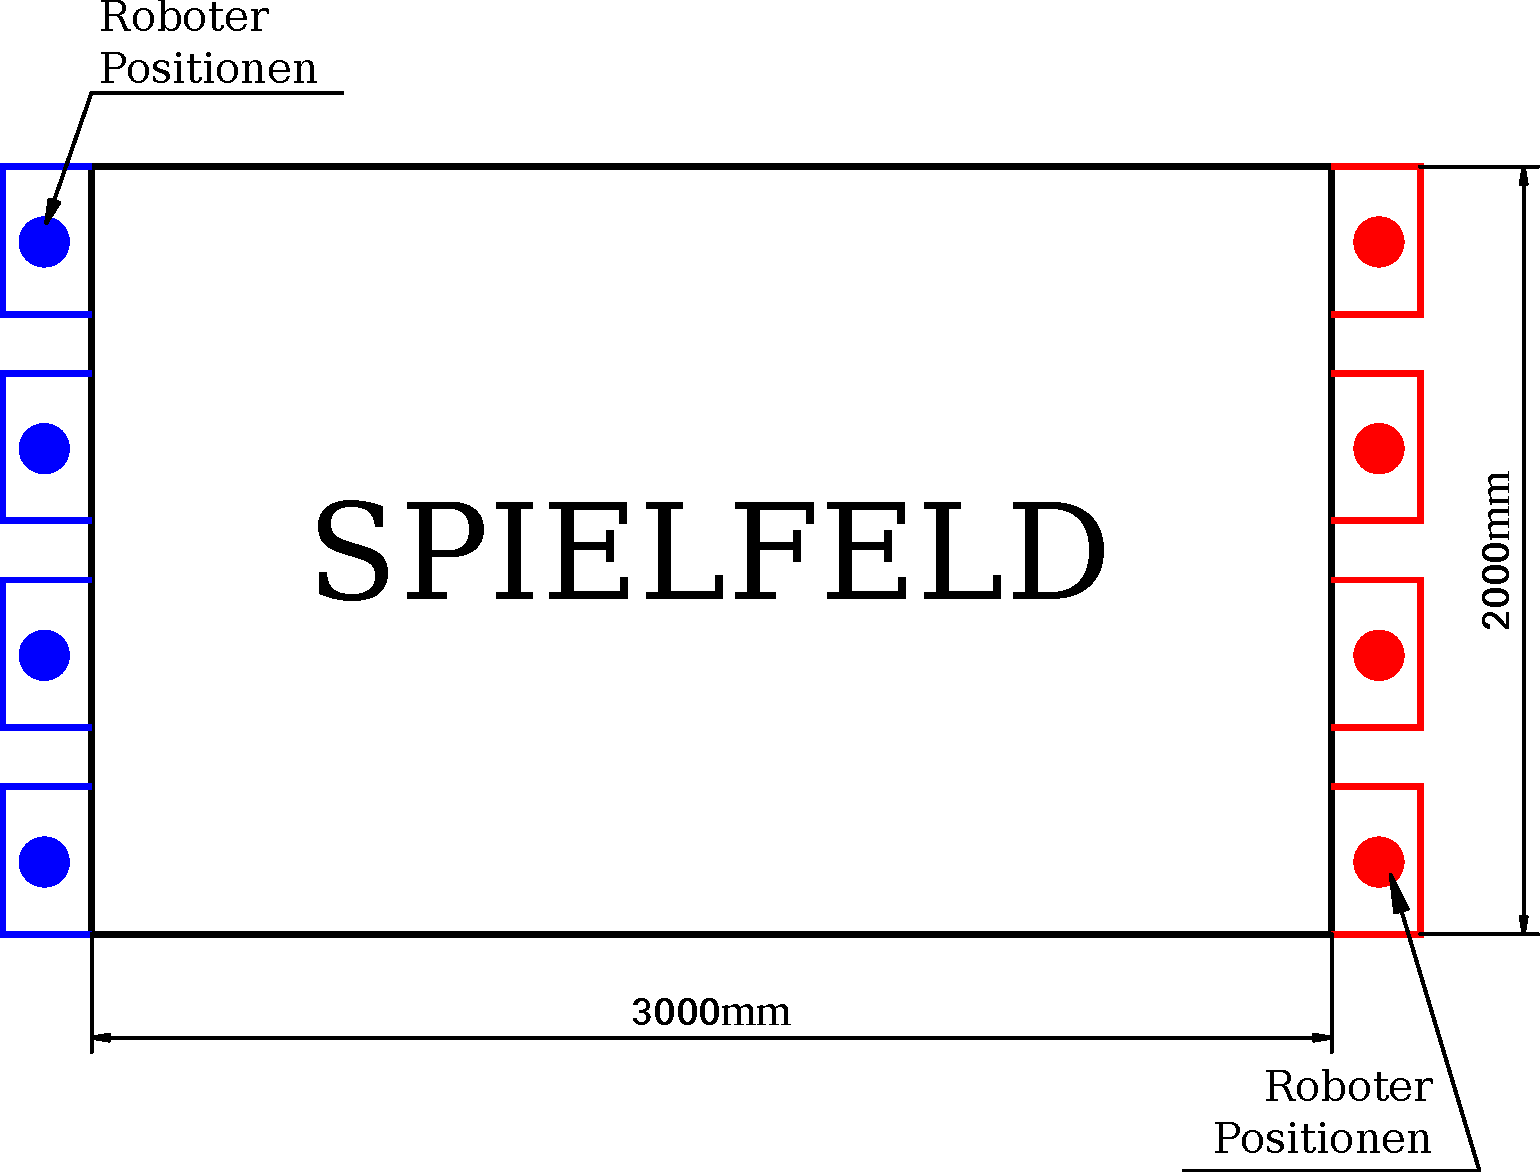
\includegraphics[width=0.8\textwidth]{Bilder/Spielfeld_2.pdf}
\end{center}
Es werden pro Gruppe 4 Roboter auf dem Spielfeld an ihre Startpositionen platziert.
Die Größe des Spielfeldes ist festgelegt.

%Alle Roboter, von beiden Teams, verbinden sich mit dem Server und übergeben diesem, dass Sie bereit sind.
%Sobald der Server das Startsignal gibt, fahren die Roboter mit einer Geschwindigkeit die $\frac{3}{4}$ der
%vollen Geschwindigkeit entspricht los.

Alle Roboter, von beiden Teams, verbinden sich mit dem Server und übergeben diesem, dass Sie bereit sind. Sobald der Server das Startsignal gibt, fahren alle Roboter los.

Dann versuchen sich die Roboter, der beiden Teams, gegenseitig zu fangen. Dazu muss einer der beiden Taster, welche am hinteren Ende des Roboters angebracht sind, betätigt werden.

%Befindet sich ein gegnerischer Roboter im Abstand X vor einem anderer Roboter, so wird die maximale Geschwindigkeit des hinteren Roboters freigeschaltet.

Wenn ein Roboter gefangen wurde, sendet dieser ein Signal an den Server und wird von diesem auf nicht Aktiv gesetzt.
Ist ein Roboter nicht Aktiv, so fährt dieser aus dem Spielfeld und verbleibt dort eine gewisse Zeit, bis er in's Spiel zurück kehrt.\\
\newline
Folgende Regeln wurden getroffen:
\begin{itemize}
	\item Ein Roboter darf erst losfahren, wenn der Server das Startsignal gegeben hat
	\item Ein Roboter darf sich nicht auf der Stelle drehen
	\item Ein Roboter darf nicht mit dem Rücken zur Wand stehen, da es so nicht möglich ist diesen zu fangen 
	%\item Erst ab einem Abstand X, darf die volle Geschwindigkeit zur Verfügung stehen
\end{itemize}